\documentclass[a4paper,titlepage,12pt]{article}
\usepackage[utf8]{inputenc} %Make sure all UTF8 characters work in the document
\usepackage{color}
\usepackage{graphicx}
\usepackage{titling}
\usepackage{tabularx}
\usepackage{longtable}
\usepackage[yyyymmdd]{datetime}
\usepackage[figurename=Figur]{caption}
\usepackage{pbox}
\usepackage{booktabs}

%Set page size
\usepackage{geometry}
\geometry{margin=3cm}

\renewcommand{\dateseparator}{-}
\renewcommand{\contentsname}{Innehållsförteckning}

%%%%%%%%%%%%%%%%%%%%%%%%%%%%%%%
% Header and footer
%%%%%%%%%%%%%%%%%%%%%%%%%%%%%%%
\usepackage{fancyhdr}
\pagestyle{fancy}

\lhead{
\includegraphics[width=0.15\linewidth]{../images/logo_full.png}}
\chead{Systemskiss för sexbent robot}
\rhead{\today}
\setlength\headheight{26pt} 

\lfoot{TSEA29 --- KMM \\ LIPS Systemskiss}
\rfoot{Grupp 9 \\ LiTHe Hex}

\pretitle{%
    \begin{center}
        \LARGE
        
\includegraphics[width=6cm]{../images/logo_full.png}\\[\bigskipamount]
}

\posttitle{\end{center}}

\begin{document}
    \title{\LARGE
        \textbf{Systemskiss för sexbent robot} \\
        \vspace*{0.5\baselineskip}
        \large
        Redaktör Frans Skarman \\
        Grupp 9 \\
        \small
        \vspace*{0.5\baselineskip}
        Version 0.1}

    \date{\today}

	\maketitle
	
	\newpage
	
	\begin{center}

		%%%%%%%%%%%%%%%%%%%%%%%%%%%%%%%%%%%%%%%%%%%%%%%%%%%%%%%%%%%%%%%%%%%%%%%%%%%%%%%%%
		%						Medlemmar
		%%%%%%%%%%%%%%%%%%%%%%%%%%%%%%%%%%%%%%%%%%%%%%%%%%%%%%%%%%%%%%%%%%%%%%%%%%%%%%%%%

		\section*{Projektidentitet}
		Grupp 9, Ht 2016, LiTHe Hex

		Linköpings Tekniska Högskola, ISY

		\begin{table}[h]
			\begin{center}
				\begin{tabular}[pos]{ l l l }
					\textbf{Namn} & \textbf{Ansvar} & \textbf{E-post} \\ \midrule
					Emil Segerbäck & Webbgränssnitt & emise935@student.liu.se \\ \midrule
					Frans Skarman & Dokumentansvarig & frask812@student.liu.se \\ \midrule
					Hannes Tuhkala & & hantu447@student.liu.se \\ \midrule
					Malcolm Vigren & Projektledare & malvi108@student.liu.se \\ \midrule
					Noak Ringman &  & noari093@student.liu.se \\ \midrule
					Olav Övrebö &  & olaov121@student.liu.se \\ \midrule
					Robin Sliwa &  & robsl733@student.liu.se \\
				\end{tabular}
			\end{center}
		\end{table}

		\centering
		\textbf{Kursansvarig}: Tomas Svensson Rum 3B:528 013--28 13 68 tomas.svensson@liu.se

		\newpage
		\tableofcontents
		\newpage


		%%%%%%%%%%%%%%%%%%%%%%%%%%%%%%%%%%%%%%%%%%%%%%%%%%%%%%%%%%%%%%%%%%%%%%%%%%%%%%%%%
		%						Historik
		%%%%%%%%%%%%%%%%%%%%%%%%%%%%%%%%%%%%%%%%%%%%%%%%%%%%%%%%%%%%%%%%%%%%%%%%%%%%%%%%%

		\section*{Dokumenthistorik}
		\begin{table}[h]
			\begin{tabular}[pos]{ l l l l l }
				\textbf{Version} & \textbf{Datum} & \textbf{Utförda förändringar} 
				& \textbf{Utförda av} & \textbf{Granskad} \\ \midrule

				0.1 & 2016--09--09 & Första utkastet & Projektgruppen & \\

			\end{tabular}
		\end{table}
	\end{center}

	%%%%%%%%%%%%%%%%%%%%%%%%%%%%%%%%%%%%%%%%%%%%%%%%%%%%%%%%%%%%%%%%%%%%%%%%%%%%%%%%%
	%						Inledning
	%%%%%%%%%%%%%%%%%%%%%%%%%%%%%%%%%%%%%%%%%%%%%%%%%%%%%%%%%%%%%%%%%%%%%%%%%%%%%%%%%

	\newpage

	\section{Inledning}
	I detta dokument beskrivs funktionaliteten produkten ska ha vid leverans.
    All funktionalitet har strukturerats i olika krav där det blir tydligt om
    kravet är uppfyllt eller inte. Krav har olika nivåer där nivå 1 är ska-krav
    som måste ha uppfyllts vid leverans. Nivå 2 ses som bör-krav och uppfylls i
    mån av tid.

	%%%%%%%%%%%%%%%%%%%%%%%%%%%%%%%%%%%%%%%%%%%%%%%%%%%%%%%%%%%%%%%%%%%%%%%%%%%%%%%%%
	%						Översikt
	%%%%%%%%%%%%%%%%%%%%%%%%%%%%%%%%%%%%%%%%%%%%%%%%%%%%%%%%%%%%%%%%%%%%%%%%%%%%%%%%%

  \newpage
	\section{Systemöversikt}
	Systemet ska innehålla tre enheter. En centralenhet för kommunikation med en
    dator, en motorikenhet som sköter hur benen rör sig samt en sensorenhet som
    tolkar sensordata. Centralenheten är även den enhet som tar beslut och
    kommunicerar med de andra enheterna. Se Figur. 1 för en översiktsbild av
    systemet.
	\begin{figure}[h]
		\centering
		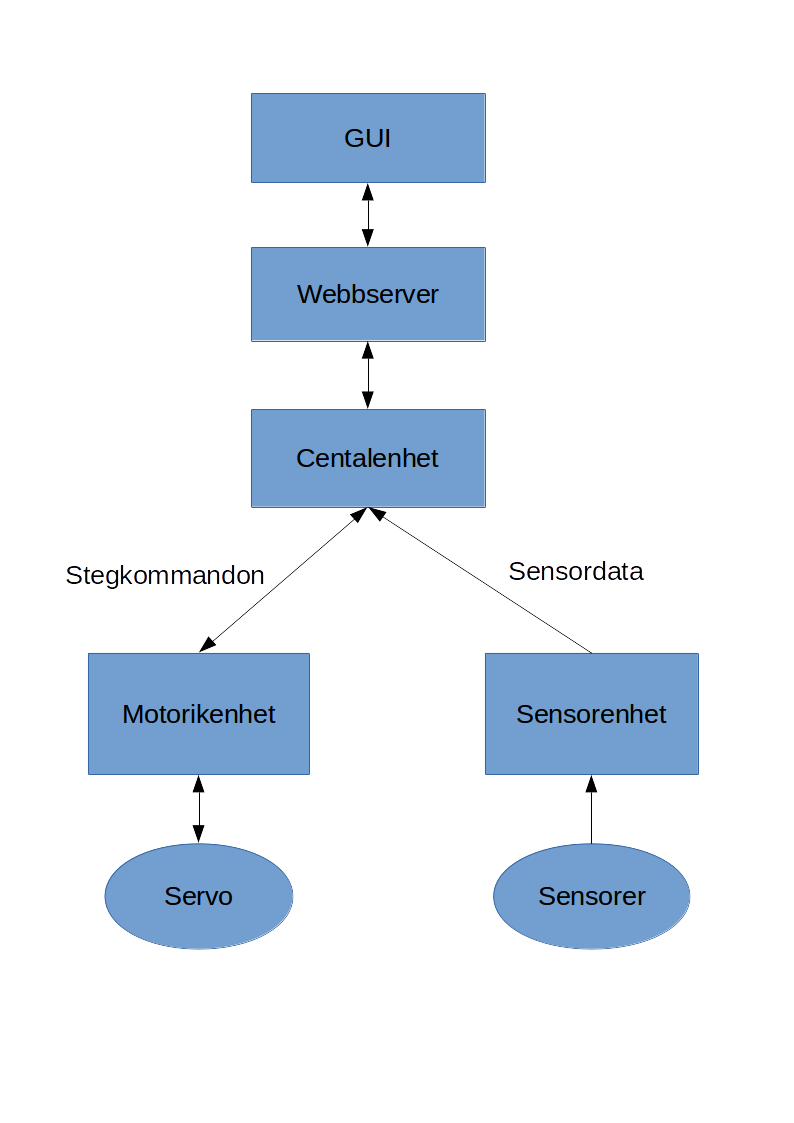
\includegraphics[width=0.5\linewidth]{../images/overview.png}
		\caption{Översikt av systemet\label{fig:overview}}
	\end{figure}

	\subsection{Kommunikation mellan enheterna}
	Kommunikation kan ske med UART, SPI eller I2C. AVR-processorerna har
	2 UART-, 3 SPI- och en I2C-ingång medan Raspberry PIen har 1 UART-, 2 SPI- och
	en I2C-ingång. 

	\subsubsection{Förslag 1}
	Om vi vill ha en LIDAR-avståndsmätare kommer sensorenhetens I2C-port att gå åt
	till kommunikation med avståndsmätaren. Sensorenheten måste alltså kommunicera med
	centralenheten med UART eller SPI.

	

	\subsection{Grov beskrivning av systemet}
	Här var det text här var det text här var det text
	här var det text här var det text här var det text
	här var det text här var det text här var det text.
	
	
	\subsection{Ingående delsystem}
	Här var det text här var det text här var det text
	här var det text här var det text här var det text
	här var det text här var det text här var det text.
	
	
	\section{Centralenheten}
	Centralenheten har 4 huvudsyften: navigation/beslutsfattning, hinderdetektion samt
	kommunikation med omvärlden.

	\subsection{Navigation och beslutsfattning}

	\subsection{Hinderdetektion}

	\subsection{Kommunikation}



	%%%%%%%%%%%%%%%%%%%%%%%%%%%%%%%%%%%%%%%%%%%%%%%%%%%%%%%%%%%%%%%%%%%%%%%%%%%%%%%%%
	%						Motorikenheten
	%%%%%%%%%%%%%%%%%%%%%%%%%%%%%%%%%%%%%%%%%%%%%%%%%%%%%%%%%%%%%%%%%%%%%%%%%%%%%%%%%
	
	\section{Motorikenheten}
	Här var det text här var det text här var det text
	här var det text här var det text här var det text
	här var det text här var det text här var det text.
	
	
	%%%%%%%%%%%%%%%%%%%%%%%%%%%%%%%%%%%%%%%%%%%%%%%%%%%%%%%%%%%%%%%%%%%%%%%%%%%%%%%%%
	%						Sensorenheten
	%%%%%%%%%%%%%%%%%%%%%%%%%%%%%%%%%%%%%%%%%%%%%%%%%%%%%%%%%%%%%%%%%%%%%%%%%%%%%%%%%
	\section{Sensorenheten}
    
    Sensorenheten är den enhet som ger roboten sinnen för omvärlden, så att den
    kan navigera autonomt genom labyrinten. Sensorenheten ska för
    centralenheten vara ett abstrakt gränssnitt till sensorerna. Centralenheten
    behöver alltså inte veta exakt vilka sensorer som används, utan istället
    läser av data som "avstånd till vägg", eller "vridning relativt väggarna".

    \subsection{Gyro}
    
    Sensorenheten ska använda ett gyro för att mäta vridning i det horizontella
    planet. Detta är användbart bland annat för att roboten ska veta hur mycket
    den ska rotera när den svänger.
    
    \subsection{Avståndssensorer fram}
    
    Sensorenheten ska använda avståndssensorer på framsidan, en sensor för att
    upptäcka väggar, och en sensor, snett vinklat ner mot golvet, för hinderdetektion. 

    Avståndssensorn som mäter framåt ska utgöras av en IR-sensor, med
    tillräckling räckvidd för att kunna avgöra om det den tittar på är en
    återvändsgränd eller inte, utan att först behöva gå in i den eventuella
    återvändsgränden.

    \subsubsection{Sensor för hinderdetektion - förslag 1}

    Sensorn som ska upptäcka hinder ska utgöras av en IR-sensor. Detta
    har fördelen av att ha samma gränssnitt som de andra IR-sensorerna roboten
    ska använda.

    \subsubsection{Sensor för hinderdetektion - förslag 2}

    Sensorn för hinderdetektion utgörs av en laser-sensor (LIDAR). Denna har
    fördelen av att vara mycket mer exakt än en IR-sensor, men nackdelen av att
    ha ett \itc-gränssnitt som ingen annan sensor har, som ökar
    komplexiteten hos sensorenheten.

    \subsection{Avståndssensorer åt sidorna}
    Roboten ska ha avståndssensorer på vardera långsida av roboten, för
    detektion av väggar och återvändsgränder.

    \subsubsection{Väggsensorer - förslag 1}
    
    En ultraljudssensor på vardera sida. Denna sensortyp har fördelen av att ha
    räckvidden 3 cm till 3 m, vilket borde ge god precision för både upptäckt
    av väggar samt återvändsgränder.

    \subsubsection{Väggsensorer - förslag 2}

    En IR-sensor på vardera sida. Denna typ har fördelen av att vara mer exakta
    än ultraljudssensorer, men har smalare räckviddsområde.

    \subsubsection{Väggsensorer - förslag 3}

    

    \subsection{Styrenhet}

    Styrenheten för sensorenheten ska bestå av en AVR-processor, som läser av och behandlar
    informationen från robotens sensorer. Styrenheten sköter även
    kommunikationen med centralenheten - den tar emot förfrågningar om data och
    skickar behandlad data på begäran.

    Styrenheten ska behandla den råa sensordatan till den grad att
    centralenheten inte behöver allt för mycket egna beräkningar på
    sensorinformationen. Den ska därför bland annat sköta brusreducering av
    datan, samt beräkna integralen av informationen från gyrot för att få ut en
    faktisk vinkel som roboten roterat. Om två avståndssensorer på vardera sida
    av roboten ska användas, ska styrenheten även beräkna robotens relativa
    orientering till väggen.
    

\end{document}
